% Created by tikzDevice version 0.12.3.1 on 2021-11-30 09:23:25
% !TEX encoding = UTF-8 Unicode
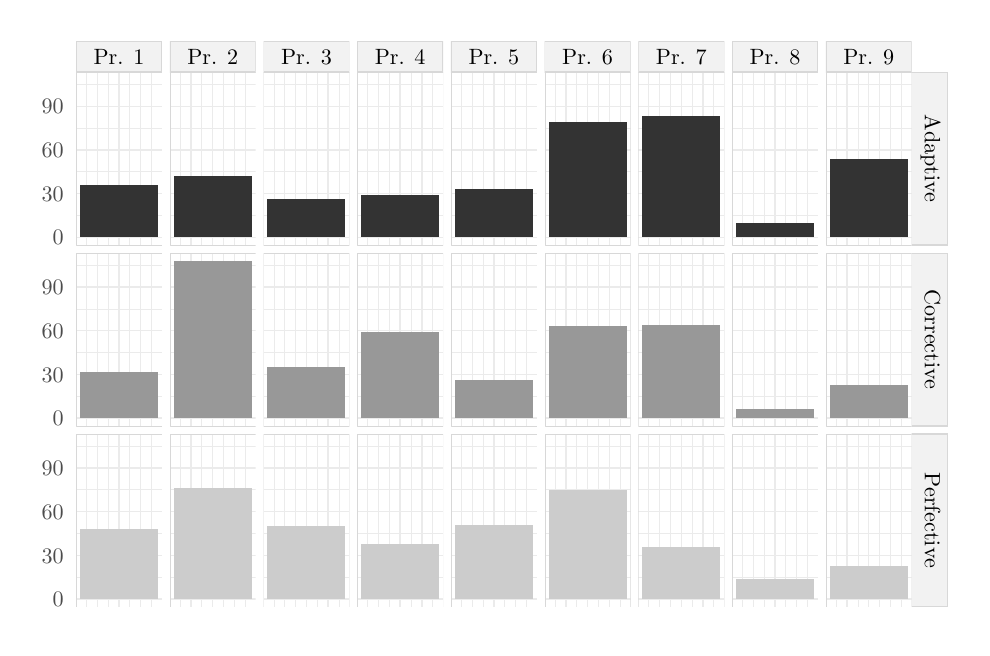
\begin{tikzpicture}[x=1pt,y=1pt]
\definecolor{fillColor}{RGB}{255,255,255}
\path[use as bounding box,fill=fillColor,fill opacity=0.00] (0,0) rectangle (337.50,216.81);
\begin{scope}
\path[clip] ( 17.50,138.23) rectangle ( 48.52,200.75);
\definecolor{drawColor}{gray}{0.92}

\path[draw=drawColor,line width= 0.3pt,line join=round] ( 17.50,148.96) --
	( 48.52,148.96);

\path[draw=drawColor,line width= 0.3pt,line join=round] ( 17.50,164.75) --
	( 48.52,164.75);

\path[draw=drawColor,line width= 0.3pt,line join=round] ( 17.50,180.54) --
	( 48.52,180.54);

\path[draw=drawColor,line width= 0.3pt,line join=round] ( 17.50,196.32) --
	( 48.52,196.32);

\path[draw=drawColor,line width= 0.3pt,line join=round] ( 21.26,138.23) --
	( 21.26,200.75);

\path[draw=drawColor,line width= 0.3pt,line join=round] ( 29.09,138.23) --
	( 29.09,200.75);

\path[draw=drawColor,line width= 0.3pt,line join=round] ( 36.92,138.23) --
	( 36.92,200.75);

\path[draw=drawColor,line width= 0.3pt,line join=round] ( 44.76,138.23) --
	( 44.76,200.75);

\path[draw=drawColor,line width= 0.5pt,line join=round] ( 17.50,141.07) --
	( 48.52,141.07);

\path[draw=drawColor,line width= 0.5pt,line join=round] ( 17.50,156.86) --
	( 48.52,156.86);

\path[draw=drawColor,line width= 0.5pt,line join=round] ( 17.50,172.64) --
	( 48.52,172.64);

\path[draw=drawColor,line width= 0.5pt,line join=round] ( 17.50,188.43) --
	( 48.52,188.43);

\path[draw=drawColor,line width= 0.5pt,line join=round] ( 25.17,138.23) --
	( 25.17,200.75);

\path[draw=drawColor,line width= 0.5pt,line join=round] ( 33.01,138.23) --
	( 33.01,200.75);

\path[draw=drawColor,line width= 0.5pt,line join=round] ( 40.84,138.23) --
	( 40.84,200.75);
\definecolor{fillColor}{gray}{0.20}

\path[fill=fillColor] ( 18.91,141.07) rectangle ( 47.11,160.01);
\definecolor{drawColor}{RGB}{216,216,216}

\path[draw=drawColor,line width= 0.1pt,line join=round,line cap=round] ( 17.50,138.23) rectangle ( 48.52,200.75);
\end{scope}
\begin{scope}
\path[clip] ( 17.50, 72.86) rectangle ( 48.52,135.38);
\definecolor{drawColor}{gray}{0.92}

\path[draw=drawColor,line width= 0.3pt,line join=round] ( 17.50, 83.60) --
	( 48.52, 83.60);

\path[draw=drawColor,line width= 0.3pt,line join=round] ( 17.50, 99.39) --
	( 48.52, 99.39);

\path[draw=drawColor,line width= 0.3pt,line join=round] ( 17.50,115.17) --
	( 48.52,115.17);

\path[draw=drawColor,line width= 0.3pt,line join=round] ( 17.50,130.96) --
	( 48.52,130.96);

\path[draw=drawColor,line width= 0.3pt,line join=round] ( 21.26, 72.86) --
	( 21.26,135.38);

\path[draw=drawColor,line width= 0.3pt,line join=round] ( 29.09, 72.86) --
	( 29.09,135.38);

\path[draw=drawColor,line width= 0.3pt,line join=round] ( 36.92, 72.86) --
	( 36.92,135.38);

\path[draw=drawColor,line width= 0.3pt,line join=round] ( 44.76, 72.86) --
	( 44.76,135.38);

\path[draw=drawColor,line width= 0.5pt,line join=round] ( 17.50, 75.71) --
	( 48.52, 75.71);

\path[draw=drawColor,line width= 0.5pt,line join=round] ( 17.50, 91.49) --
	( 48.52, 91.49);

\path[draw=drawColor,line width= 0.5pt,line join=round] ( 17.50,107.28) --
	( 48.52,107.28);

\path[draw=drawColor,line width= 0.5pt,line join=round] ( 17.50,123.07) --
	( 48.52,123.07);

\path[draw=drawColor,line width= 0.5pt,line join=round] ( 25.17, 72.86) --
	( 25.17,135.38);

\path[draw=drawColor,line width= 0.5pt,line join=round] ( 33.01, 72.86) --
	( 33.01,135.38);

\path[draw=drawColor,line width= 0.5pt,line join=round] ( 40.84, 72.86) --
	( 40.84,135.38);
\definecolor{fillColor}{RGB}{152,152,152}

\path[fill=fillColor] ( 18.91, 75.71) rectangle ( 47.11, 92.55);
\definecolor{drawColor}{RGB}{216,216,216}

\path[draw=drawColor,line width= 0.1pt,line join=round,line cap=round] ( 17.50, 72.86) rectangle ( 48.52,135.38);
\end{scope}
\begin{scope}
\path[clip] ( 17.50,  7.50) rectangle ( 48.52, 70.02);
\definecolor{drawColor}{gray}{0.92}

\path[draw=drawColor,line width= 0.3pt,line join=round] ( 17.50, 18.24) --
	( 48.52, 18.24);

\path[draw=drawColor,line width= 0.3pt,line join=round] ( 17.50, 34.02) --
	( 48.52, 34.02);

\path[draw=drawColor,line width= 0.3pt,line join=round] ( 17.50, 49.81) --
	( 48.52, 49.81);

\path[draw=drawColor,line width= 0.3pt,line join=round] ( 17.50, 65.60) --
	( 48.52, 65.60);

\path[draw=drawColor,line width= 0.3pt,line join=round] ( 21.26,  7.50) --
	( 21.26, 70.02);

\path[draw=drawColor,line width= 0.3pt,line join=round] ( 29.09,  7.50) --
	( 29.09, 70.02);

\path[draw=drawColor,line width= 0.3pt,line join=round] ( 36.92,  7.50) --
	( 36.92, 70.02);

\path[draw=drawColor,line width= 0.3pt,line join=round] ( 44.76,  7.50) --
	( 44.76, 70.02);

\path[draw=drawColor,line width= 0.5pt,line join=round] ( 17.50, 10.34) --
	( 48.52, 10.34);

\path[draw=drawColor,line width= 0.5pt,line join=round] ( 17.50, 26.13) --
	( 48.52, 26.13);

\path[draw=drawColor,line width= 0.5pt,line join=round] ( 17.50, 41.92) --
	( 48.52, 41.92);

\path[draw=drawColor,line width= 0.5pt,line join=round] ( 17.50, 57.70) --
	( 48.52, 57.70);

\path[draw=drawColor,line width= 0.5pt,line join=round] ( 25.17,  7.50) --
	( 25.17, 70.02);

\path[draw=drawColor,line width= 0.5pt,line join=round] ( 33.01,  7.50) --
	( 33.01, 70.02);

\path[draw=drawColor,line width= 0.5pt,line join=round] ( 40.84,  7.50) --
	( 40.84, 70.02);
\definecolor{fillColor}{gray}{0.80}

\path[fill=fillColor] ( 18.91, 10.34) rectangle ( 47.11, 35.60);
\definecolor{drawColor}{RGB}{216,216,216}

\path[draw=drawColor,line width= 0.1pt,line join=round,line cap=round] ( 17.50,  7.50) rectangle ( 48.52, 70.02);
\end{scope}
\begin{scope}
\path[clip] ( 51.36,138.23) rectangle ( 82.38,200.75);
\definecolor{drawColor}{gray}{0.92}

\path[draw=drawColor,line width= 0.3pt,line join=round] ( 51.36,148.96) --
	( 82.38,148.96);

\path[draw=drawColor,line width= 0.3pt,line join=round] ( 51.36,164.75) --
	( 82.38,164.75);

\path[draw=drawColor,line width= 0.3pt,line join=round] ( 51.36,180.54) --
	( 82.38,180.54);

\path[draw=drawColor,line width= 0.3pt,line join=round] ( 51.36,196.32) --
	( 82.38,196.32);

\path[draw=drawColor,line width= 0.3pt,line join=round] ( 55.12,138.23) --
	( 55.12,200.75);

\path[draw=drawColor,line width= 0.3pt,line join=round] ( 62.96,138.23) --
	( 62.96,200.75);

\path[draw=drawColor,line width= 0.3pt,line join=round] ( 70.79,138.23) --
	( 70.79,200.75);

\path[draw=drawColor,line width= 0.3pt,line join=round] ( 78.62,138.23) --
	( 78.62,200.75);

\path[draw=drawColor,line width= 0.5pt,line join=round] ( 51.36,141.07) --
	( 82.38,141.07);

\path[draw=drawColor,line width= 0.5pt,line join=round] ( 51.36,156.86) --
	( 82.38,156.86);

\path[draw=drawColor,line width= 0.5pt,line join=round] ( 51.36,172.64) --
	( 82.38,172.64);

\path[draw=drawColor,line width= 0.5pt,line join=round] ( 51.36,188.43) --
	( 82.38,188.43);

\path[draw=drawColor,line width= 0.5pt,line join=round] ( 59.04,138.23) --
	( 59.04,200.75);

\path[draw=drawColor,line width= 0.5pt,line join=round] ( 66.87,138.23) --
	( 66.87,200.75);

\path[draw=drawColor,line width= 0.5pt,line join=round] ( 74.71,138.23) --
	( 74.71,200.75);
\definecolor{fillColor}{gray}{0.20}

\path[fill=fillColor] ( 52.77,141.07) rectangle ( 80.97,163.17);
\definecolor{drawColor}{RGB}{216,216,216}

\path[draw=drawColor,line width= 0.1pt,line join=round,line cap=round] ( 51.36,138.23) rectangle ( 82.38,200.75);
\end{scope}
\begin{scope}
\path[clip] ( 51.36, 72.86) rectangle ( 82.38,135.38);
\definecolor{drawColor}{gray}{0.92}

\path[draw=drawColor,line width= 0.3pt,line join=round] ( 51.36, 83.60) --
	( 82.38, 83.60);

\path[draw=drawColor,line width= 0.3pt,line join=round] ( 51.36, 99.39) --
	( 82.38, 99.39);

\path[draw=drawColor,line width= 0.3pt,line join=round] ( 51.36,115.17) --
	( 82.38,115.17);

\path[draw=drawColor,line width= 0.3pt,line join=round] ( 51.36,130.96) --
	( 82.38,130.96);

\path[draw=drawColor,line width= 0.3pt,line join=round] ( 55.12, 72.86) --
	( 55.12,135.38);

\path[draw=drawColor,line width= 0.3pt,line join=round] ( 62.96, 72.86) --
	( 62.96,135.38);

\path[draw=drawColor,line width= 0.3pt,line join=round] ( 70.79, 72.86) --
	( 70.79,135.38);

\path[draw=drawColor,line width= 0.3pt,line join=round] ( 78.62, 72.86) --
	( 78.62,135.38);

\path[draw=drawColor,line width= 0.5pt,line join=round] ( 51.36, 75.71) --
	( 82.38, 75.71);

\path[draw=drawColor,line width= 0.5pt,line join=round] ( 51.36, 91.49) --
	( 82.38, 91.49);

\path[draw=drawColor,line width= 0.5pt,line join=round] ( 51.36,107.28) --
	( 82.38,107.28);

\path[draw=drawColor,line width= 0.5pt,line join=round] ( 51.36,123.07) --
	( 82.38,123.07);

\path[draw=drawColor,line width= 0.5pt,line join=round] ( 59.04, 72.86) --
	( 59.04,135.38);

\path[draw=drawColor,line width= 0.5pt,line join=round] ( 66.87, 72.86) --
	( 66.87,135.38);

\path[draw=drawColor,line width= 0.5pt,line join=round] ( 74.71, 72.86) --
	( 74.71,135.38);
\definecolor{fillColor}{RGB}{152,152,152}

\path[fill=fillColor] ( 52.77, 75.71) rectangle ( 80.97,132.54);
\definecolor{drawColor}{RGB}{216,216,216}

\path[draw=drawColor,line width= 0.1pt,line join=round,line cap=round] ( 51.36, 72.86) rectangle ( 82.38,135.38);
\end{scope}
\begin{scope}
\path[clip] ( 51.36,  7.50) rectangle ( 82.38, 70.02);
\definecolor{drawColor}{gray}{0.92}

\path[draw=drawColor,line width= 0.3pt,line join=round] ( 51.36, 18.24) --
	( 82.38, 18.24);

\path[draw=drawColor,line width= 0.3pt,line join=round] ( 51.36, 34.02) --
	( 82.38, 34.02);

\path[draw=drawColor,line width= 0.3pt,line join=round] ( 51.36, 49.81) --
	( 82.38, 49.81);

\path[draw=drawColor,line width= 0.3pt,line join=round] ( 51.36, 65.60) --
	( 82.38, 65.60);

\path[draw=drawColor,line width= 0.3pt,line join=round] ( 55.12,  7.50) --
	( 55.12, 70.02);

\path[draw=drawColor,line width= 0.3pt,line join=round] ( 62.96,  7.50) --
	( 62.96, 70.02);

\path[draw=drawColor,line width= 0.3pt,line join=round] ( 70.79,  7.50) --
	( 70.79, 70.02);

\path[draw=drawColor,line width= 0.3pt,line join=round] ( 78.62,  7.50) --
	( 78.62, 70.02);

\path[draw=drawColor,line width= 0.5pt,line join=round] ( 51.36, 10.34) --
	( 82.38, 10.34);

\path[draw=drawColor,line width= 0.5pt,line join=round] ( 51.36, 26.13) --
	( 82.38, 26.13);

\path[draw=drawColor,line width= 0.5pt,line join=round] ( 51.36, 41.92) --
	( 82.38, 41.92);

\path[draw=drawColor,line width= 0.5pt,line join=round] ( 51.36, 57.70) --
	( 82.38, 57.70);

\path[draw=drawColor,line width= 0.5pt,line join=round] ( 59.04,  7.50) --
	( 59.04, 70.02);

\path[draw=drawColor,line width= 0.5pt,line join=round] ( 66.87,  7.50) --
	( 66.87, 70.02);

\path[draw=drawColor,line width= 0.5pt,line join=round] ( 74.71,  7.50) --
	( 74.71, 70.02);
\definecolor{fillColor}{gray}{0.80}

\path[fill=fillColor] ( 52.77, 10.34) rectangle ( 80.97, 50.34);
\definecolor{drawColor}{RGB}{216,216,216}

\path[draw=drawColor,line width= 0.1pt,line join=round,line cap=round] ( 51.36,  7.50) rectangle ( 82.38, 70.02);
\end{scope}
\begin{scope}
\path[clip] ( 85.23,138.23) rectangle (116.25,200.75);
\definecolor{drawColor}{gray}{0.92}

\path[draw=drawColor,line width= 0.3pt,line join=round] ( 85.23,148.96) --
	(116.25,148.96);

\path[draw=drawColor,line width= 0.3pt,line join=round] ( 85.23,164.75) --
	(116.25,164.75);

\path[draw=drawColor,line width= 0.3pt,line join=round] ( 85.23,180.54) --
	(116.25,180.54);

\path[draw=drawColor,line width= 0.3pt,line join=round] ( 85.23,196.32) --
	(116.25,196.32);

\path[draw=drawColor,line width= 0.3pt,line join=round] ( 88.99,138.23) --
	( 88.99,200.75);

\path[draw=drawColor,line width= 0.3pt,line join=round] ( 96.82,138.23) --
	( 96.82,200.75);

\path[draw=drawColor,line width= 0.3pt,line join=round] (104.65,138.23) --
	(104.65,200.75);

\path[draw=drawColor,line width= 0.3pt,line join=round] (112.49,138.23) --
	(112.49,200.75);

\path[draw=drawColor,line width= 0.5pt,line join=round] ( 85.23,141.07) --
	(116.25,141.07);

\path[draw=drawColor,line width= 0.5pt,line join=round] ( 85.23,156.86) --
	(116.25,156.86);

\path[draw=drawColor,line width= 0.5pt,line join=round] ( 85.23,172.64) --
	(116.25,172.64);

\path[draw=drawColor,line width= 0.5pt,line join=round] ( 85.23,188.43) --
	(116.25,188.43);

\path[draw=drawColor,line width= 0.5pt,line join=round] ( 92.90,138.23) --
	( 92.90,200.75);

\path[draw=drawColor,line width= 0.5pt,line join=round] (100.74,138.23) --
	(100.74,200.75);

\path[draw=drawColor,line width= 0.5pt,line join=round] (108.57,138.23) --
	(108.57,200.75);
\definecolor{fillColor}{gray}{0.20}

\path[fill=fillColor] ( 86.64,141.07) rectangle (114.84,154.75);
\definecolor{drawColor}{RGB}{216,216,216}

\path[draw=drawColor,line width= 0.1pt,line join=round,line cap=round] ( 85.23,138.23) rectangle (116.25,200.75);
\end{scope}
\begin{scope}
\path[clip] ( 85.23, 72.86) rectangle (116.25,135.38);
\definecolor{drawColor}{gray}{0.92}

\path[draw=drawColor,line width= 0.3pt,line join=round] ( 85.23, 83.60) --
	(116.25, 83.60);

\path[draw=drawColor,line width= 0.3pt,line join=round] ( 85.23, 99.39) --
	(116.25, 99.39);

\path[draw=drawColor,line width= 0.3pt,line join=round] ( 85.23,115.17) --
	(116.25,115.17);

\path[draw=drawColor,line width= 0.3pt,line join=round] ( 85.23,130.96) --
	(116.25,130.96);

\path[draw=drawColor,line width= 0.3pt,line join=round] ( 88.99, 72.86) --
	( 88.99,135.38);

\path[draw=drawColor,line width= 0.3pt,line join=round] ( 96.82, 72.86) --
	( 96.82,135.38);

\path[draw=drawColor,line width= 0.3pt,line join=round] (104.65, 72.86) --
	(104.65,135.38);

\path[draw=drawColor,line width= 0.3pt,line join=round] (112.49, 72.86) --
	(112.49,135.38);

\path[draw=drawColor,line width= 0.5pt,line join=round] ( 85.23, 75.71) --
	(116.25, 75.71);

\path[draw=drawColor,line width= 0.5pt,line join=round] ( 85.23, 91.49) --
	(116.25, 91.49);

\path[draw=drawColor,line width= 0.5pt,line join=round] ( 85.23,107.28) --
	(116.25,107.28);

\path[draw=drawColor,line width= 0.5pt,line join=round] ( 85.23,123.07) --
	(116.25,123.07);

\path[draw=drawColor,line width= 0.5pt,line join=round] ( 92.90, 72.86) --
	( 92.90,135.38);

\path[draw=drawColor,line width= 0.5pt,line join=round] (100.74, 72.86) --
	(100.74,135.38);

\path[draw=drawColor,line width= 0.5pt,line join=round] (108.57, 72.86) --
	(108.57,135.38);
\definecolor{fillColor}{RGB}{152,152,152}

\path[fill=fillColor] ( 86.64, 75.71) rectangle (114.84, 94.12);
\definecolor{drawColor}{RGB}{216,216,216}

\path[draw=drawColor,line width= 0.1pt,line join=round,line cap=round] ( 85.23, 72.86) rectangle (116.25,135.38);
\end{scope}
\begin{scope}
\path[clip] ( 85.23,  7.50) rectangle (116.25, 70.02);
\definecolor{drawColor}{gray}{0.92}

\path[draw=drawColor,line width= 0.3pt,line join=round] ( 85.23, 18.24) --
	(116.25, 18.24);

\path[draw=drawColor,line width= 0.3pt,line join=round] ( 85.23, 34.02) --
	(116.25, 34.02);

\path[draw=drawColor,line width= 0.3pt,line join=round] ( 85.23, 49.81) --
	(116.25, 49.81);

\path[draw=drawColor,line width= 0.3pt,line join=round] ( 85.23, 65.60) --
	(116.25, 65.60);

\path[draw=drawColor,line width= 0.3pt,line join=round] ( 88.99,  7.50) --
	( 88.99, 70.02);

\path[draw=drawColor,line width= 0.3pt,line join=round] ( 96.82,  7.50) --
	( 96.82, 70.02);

\path[draw=drawColor,line width= 0.3pt,line join=round] (104.65,  7.50) --
	(104.65, 70.02);

\path[draw=drawColor,line width= 0.3pt,line join=round] (112.49,  7.50) --
	(112.49, 70.02);

\path[draw=drawColor,line width= 0.5pt,line join=round] ( 85.23, 10.34) --
	(116.25, 10.34);

\path[draw=drawColor,line width= 0.5pt,line join=round] ( 85.23, 26.13) --
	(116.25, 26.13);

\path[draw=drawColor,line width= 0.5pt,line join=round] ( 85.23, 41.92) --
	(116.25, 41.92);

\path[draw=drawColor,line width= 0.5pt,line join=round] ( 85.23, 57.70) --
	(116.25, 57.70);

\path[draw=drawColor,line width= 0.5pt,line join=round] ( 92.90,  7.50) --
	( 92.90, 70.02);

\path[draw=drawColor,line width= 0.5pt,line join=round] (100.74,  7.50) --
	(100.74, 70.02);

\path[draw=drawColor,line width= 0.5pt,line join=round] (108.57,  7.50) --
	(108.57, 70.02);
\definecolor{fillColor}{gray}{0.80}

\path[fill=fillColor] ( 86.64, 10.34) rectangle (114.84, 36.65);
\definecolor{drawColor}{RGB}{216,216,216}

\path[draw=drawColor,line width= 0.1pt,line join=round,line cap=round] ( 85.23,  7.50) rectangle (116.25, 70.02);
\end{scope}
\begin{scope}
\path[clip] (119.09,138.23) rectangle (150.11,200.75);
\definecolor{drawColor}{gray}{0.92}

\path[draw=drawColor,line width= 0.3pt,line join=round] (119.09,148.96) --
	(150.11,148.96);

\path[draw=drawColor,line width= 0.3pt,line join=round] (119.09,164.75) --
	(150.11,164.75);

\path[draw=drawColor,line width= 0.3pt,line join=round] (119.09,180.54) --
	(150.11,180.54);

\path[draw=drawColor,line width= 0.3pt,line join=round] (119.09,196.32) --
	(150.11,196.32);

\path[draw=drawColor,line width= 0.3pt,line join=round] (122.85,138.23) --
	(122.85,200.75);

\path[draw=drawColor,line width= 0.3pt,line join=round] (130.69,138.23) --
	(130.69,200.75);

\path[draw=drawColor,line width= 0.3pt,line join=round] (138.52,138.23) --
	(138.52,200.75);

\path[draw=drawColor,line width= 0.3pt,line join=round] (146.35,138.23) --
	(146.35,200.75);

\path[draw=drawColor,line width= 0.5pt,line join=round] (119.09,141.07) --
	(150.11,141.07);

\path[draw=drawColor,line width= 0.5pt,line join=round] (119.09,156.86) --
	(150.11,156.86);

\path[draw=drawColor,line width= 0.5pt,line join=round] (119.09,172.64) --
	(150.11,172.64);

\path[draw=drawColor,line width= 0.5pt,line join=round] (119.09,188.43) --
	(150.11,188.43);

\path[draw=drawColor,line width= 0.5pt,line join=round] (126.77,138.23) --
	(126.77,200.75);

\path[draw=drawColor,line width= 0.5pt,line join=round] (134.60,138.23) --
	(134.60,200.75);

\path[draw=drawColor,line width= 0.5pt,line join=round] (142.44,138.23) --
	(142.44,200.75);
\definecolor{fillColor}{gray}{0.20}

\path[fill=fillColor] (120.50,141.07) rectangle (148.70,156.33);
\definecolor{drawColor}{RGB}{216,216,216}

\path[draw=drawColor,line width= 0.1pt,line join=round,line cap=round] (119.09,138.23) rectangle (150.11,200.75);
\end{scope}
\begin{scope}
\path[clip] (119.09, 72.86) rectangle (150.11,135.38);
\definecolor{drawColor}{gray}{0.92}

\path[draw=drawColor,line width= 0.3pt,line join=round] (119.09, 83.60) --
	(150.11, 83.60);

\path[draw=drawColor,line width= 0.3pt,line join=round] (119.09, 99.39) --
	(150.11, 99.39);

\path[draw=drawColor,line width= 0.3pt,line join=round] (119.09,115.17) --
	(150.11,115.17);

\path[draw=drawColor,line width= 0.3pt,line join=round] (119.09,130.96) --
	(150.11,130.96);

\path[draw=drawColor,line width= 0.3pt,line join=round] (122.85, 72.86) --
	(122.85,135.38);

\path[draw=drawColor,line width= 0.3pt,line join=round] (130.69, 72.86) --
	(130.69,135.38);

\path[draw=drawColor,line width= 0.3pt,line join=round] (138.52, 72.86) --
	(138.52,135.38);

\path[draw=drawColor,line width= 0.3pt,line join=round] (146.35, 72.86) --
	(146.35,135.38);

\path[draw=drawColor,line width= 0.5pt,line join=round] (119.09, 75.71) --
	(150.11, 75.71);

\path[draw=drawColor,line width= 0.5pt,line join=round] (119.09, 91.49) --
	(150.11, 91.49);

\path[draw=drawColor,line width= 0.5pt,line join=round] (119.09,107.28) --
	(150.11,107.28);

\path[draw=drawColor,line width= 0.5pt,line join=round] (119.09,123.07) --
	(150.11,123.07);

\path[draw=drawColor,line width= 0.5pt,line join=round] (126.77, 72.86) --
	(126.77,135.38);

\path[draw=drawColor,line width= 0.5pt,line join=round] (134.60, 72.86) --
	(134.60,135.38);

\path[draw=drawColor,line width= 0.5pt,line join=round] (142.44, 72.86) --
	(142.44,135.38);
\definecolor{fillColor}{RGB}{152,152,152}

\path[fill=fillColor] (120.50, 75.71) rectangle (148.70,106.75);
\definecolor{drawColor}{RGB}{216,216,216}

\path[draw=drawColor,line width= 0.1pt,line join=round,line cap=round] (119.09, 72.86) rectangle (150.11,135.38);
\end{scope}
\begin{scope}
\path[clip] (119.09,  7.50) rectangle (150.11, 70.02);
\definecolor{drawColor}{gray}{0.92}

\path[draw=drawColor,line width= 0.3pt,line join=round] (119.09, 18.24) --
	(150.11, 18.24);

\path[draw=drawColor,line width= 0.3pt,line join=round] (119.09, 34.02) --
	(150.11, 34.02);

\path[draw=drawColor,line width= 0.3pt,line join=round] (119.09, 49.81) --
	(150.11, 49.81);

\path[draw=drawColor,line width= 0.3pt,line join=round] (119.09, 65.60) --
	(150.11, 65.60);

\path[draw=drawColor,line width= 0.3pt,line join=round] (122.85,  7.50) --
	(122.85, 70.02);

\path[draw=drawColor,line width= 0.3pt,line join=round] (130.69,  7.50) --
	(130.69, 70.02);

\path[draw=drawColor,line width= 0.3pt,line join=round] (138.52,  7.50) --
	(138.52, 70.02);

\path[draw=drawColor,line width= 0.3pt,line join=round] (146.35,  7.50) --
	(146.35, 70.02);

\path[draw=drawColor,line width= 0.5pt,line join=round] (119.09, 10.34) --
	(150.11, 10.34);

\path[draw=drawColor,line width= 0.5pt,line join=round] (119.09, 26.13) --
	(150.11, 26.13);

\path[draw=drawColor,line width= 0.5pt,line join=round] (119.09, 41.92) --
	(150.11, 41.92);

\path[draw=drawColor,line width= 0.5pt,line join=round] (119.09, 57.70) --
	(150.11, 57.70);

\path[draw=drawColor,line width= 0.5pt,line join=round] (126.77,  7.50) --
	(126.77, 70.02);

\path[draw=drawColor,line width= 0.5pt,line join=round] (134.60,  7.50) --
	(134.60, 70.02);

\path[draw=drawColor,line width= 0.5pt,line join=round] (142.44,  7.50) --
	(142.44, 70.02);
\definecolor{fillColor}{gray}{0.80}

\path[fill=fillColor] (120.50, 10.34) rectangle (148.70, 30.34);
\definecolor{drawColor}{RGB}{216,216,216}

\path[draw=drawColor,line width= 0.1pt,line join=round,line cap=round] (119.09,  7.50) rectangle (150.11, 70.02);
\end{scope}
\begin{scope}
\path[clip] (152.96,138.23) rectangle (183.98,200.75);
\definecolor{drawColor}{gray}{0.92}

\path[draw=drawColor,line width= 0.3pt,line join=round] (152.96,148.96) --
	(183.98,148.96);

\path[draw=drawColor,line width= 0.3pt,line join=round] (152.96,164.75) --
	(183.98,164.75);

\path[draw=drawColor,line width= 0.3pt,line join=round] (152.96,180.54) --
	(183.98,180.54);

\path[draw=drawColor,line width= 0.3pt,line join=round] (152.96,196.32) --
	(183.98,196.32);

\path[draw=drawColor,line width= 0.3pt,line join=round] (156.72,138.23) --
	(156.72,200.75);

\path[draw=drawColor,line width= 0.3pt,line join=round] (164.55,138.23) --
	(164.55,200.75);

\path[draw=drawColor,line width= 0.3pt,line join=round] (172.38,138.23) --
	(172.38,200.75);

\path[draw=drawColor,line width= 0.3pt,line join=round] (180.22,138.23) --
	(180.22,200.75);

\path[draw=drawColor,line width= 0.5pt,line join=round] (152.96,141.07) --
	(183.98,141.07);

\path[draw=drawColor,line width= 0.5pt,line join=round] (152.96,156.86) --
	(183.98,156.86);

\path[draw=drawColor,line width= 0.5pt,line join=round] (152.96,172.64) --
	(183.98,172.64);

\path[draw=drawColor,line width= 0.5pt,line join=round] (152.96,188.43) --
	(183.98,188.43);

\path[draw=drawColor,line width= 0.5pt,line join=round] (160.63,138.23) --
	(160.63,200.75);

\path[draw=drawColor,line width= 0.5pt,line join=round] (168.47,138.23) --
	(168.47,200.75);

\path[draw=drawColor,line width= 0.5pt,line join=round] (176.30,138.23) --
	(176.30,200.75);
\definecolor{fillColor}{gray}{0.20}

\path[fill=fillColor] (154.37,141.07) rectangle (182.57,158.43);
\definecolor{drawColor}{RGB}{216,216,216}

\path[draw=drawColor,line width= 0.1pt,line join=round,line cap=round] (152.96,138.23) rectangle (183.98,200.75);
\end{scope}
\begin{scope}
\path[clip] (152.96, 72.86) rectangle (183.98,135.38);
\definecolor{drawColor}{gray}{0.92}

\path[draw=drawColor,line width= 0.3pt,line join=round] (152.96, 83.60) --
	(183.98, 83.60);

\path[draw=drawColor,line width= 0.3pt,line join=round] (152.96, 99.39) --
	(183.98, 99.39);

\path[draw=drawColor,line width= 0.3pt,line join=round] (152.96,115.17) --
	(183.98,115.17);

\path[draw=drawColor,line width= 0.3pt,line join=round] (152.96,130.96) --
	(183.98,130.96);

\path[draw=drawColor,line width= 0.3pt,line join=round] (156.72, 72.86) --
	(156.72,135.38);

\path[draw=drawColor,line width= 0.3pt,line join=round] (164.55, 72.86) --
	(164.55,135.38);

\path[draw=drawColor,line width= 0.3pt,line join=round] (172.38, 72.86) --
	(172.38,135.38);

\path[draw=drawColor,line width= 0.3pt,line join=round] (180.22, 72.86) --
	(180.22,135.38);

\path[draw=drawColor,line width= 0.5pt,line join=round] (152.96, 75.71) --
	(183.98, 75.71);

\path[draw=drawColor,line width= 0.5pt,line join=round] (152.96, 91.49) --
	(183.98, 91.49);

\path[draw=drawColor,line width= 0.5pt,line join=round] (152.96,107.28) --
	(183.98,107.28);

\path[draw=drawColor,line width= 0.5pt,line join=round] (152.96,123.07) --
	(183.98,123.07);

\path[draw=drawColor,line width= 0.5pt,line join=round] (160.63, 72.86) --
	(160.63,135.38);

\path[draw=drawColor,line width= 0.5pt,line join=round] (168.47, 72.86) --
	(168.47,135.38);

\path[draw=drawColor,line width= 0.5pt,line join=round] (176.30, 72.86) --
	(176.30,135.38);
\definecolor{fillColor}{RGB}{152,152,152}

\path[fill=fillColor] (154.37, 75.71) rectangle (182.57, 89.39);
\definecolor{drawColor}{RGB}{216,216,216}

\path[draw=drawColor,line width= 0.1pt,line join=round,line cap=round] (152.96, 72.86) rectangle (183.98,135.38);
\end{scope}
\begin{scope}
\path[clip] (152.96,  7.50) rectangle (183.98, 70.02);
\definecolor{drawColor}{gray}{0.92}

\path[draw=drawColor,line width= 0.3pt,line join=round] (152.96, 18.24) --
	(183.98, 18.24);

\path[draw=drawColor,line width= 0.3pt,line join=round] (152.96, 34.02) --
	(183.98, 34.02);

\path[draw=drawColor,line width= 0.3pt,line join=round] (152.96, 49.81) --
	(183.98, 49.81);

\path[draw=drawColor,line width= 0.3pt,line join=round] (152.96, 65.60) --
	(183.98, 65.60);

\path[draw=drawColor,line width= 0.3pt,line join=round] (156.72,  7.50) --
	(156.72, 70.02);

\path[draw=drawColor,line width= 0.3pt,line join=round] (164.55,  7.50) --
	(164.55, 70.02);

\path[draw=drawColor,line width= 0.3pt,line join=round] (172.38,  7.50) --
	(172.38, 70.02);

\path[draw=drawColor,line width= 0.3pt,line join=round] (180.22,  7.50) --
	(180.22, 70.02);

\path[draw=drawColor,line width= 0.5pt,line join=round] (152.96, 10.34) --
	(183.98, 10.34);

\path[draw=drawColor,line width= 0.5pt,line join=round] (152.96, 26.13) --
	(183.98, 26.13);

\path[draw=drawColor,line width= 0.5pt,line join=round] (152.96, 41.92) --
	(183.98, 41.92);

\path[draw=drawColor,line width= 0.5pt,line join=round] (152.96, 57.70) --
	(183.98, 57.70);

\path[draw=drawColor,line width= 0.5pt,line join=round] (160.63,  7.50) --
	(160.63, 70.02);

\path[draw=drawColor,line width= 0.5pt,line join=round] (168.47,  7.50) --
	(168.47, 70.02);

\path[draw=drawColor,line width= 0.5pt,line join=round] (176.30,  7.50) --
	(176.30, 70.02);
\definecolor{fillColor}{gray}{0.80}

\path[fill=fillColor] (154.37, 10.34) rectangle (182.57, 37.18);
\definecolor{drawColor}{RGB}{216,216,216}

\path[draw=drawColor,line width= 0.1pt,line join=round,line cap=round] (152.96,  7.50) rectangle (183.98, 70.02);
\end{scope}
\begin{scope}
\path[clip] (186.82,138.23) rectangle (217.84,200.75);
\definecolor{drawColor}{gray}{0.92}

\path[draw=drawColor,line width= 0.3pt,line join=round] (186.82,148.96) --
	(217.84,148.96);

\path[draw=drawColor,line width= 0.3pt,line join=round] (186.82,164.75) --
	(217.84,164.75);

\path[draw=drawColor,line width= 0.3pt,line join=round] (186.82,180.54) --
	(217.84,180.54);

\path[draw=drawColor,line width= 0.3pt,line join=round] (186.82,196.32) --
	(217.84,196.32);

\path[draw=drawColor,line width= 0.3pt,line join=round] (190.58,138.23) --
	(190.58,200.75);

\path[draw=drawColor,line width= 0.3pt,line join=round] (198.42,138.23) --
	(198.42,200.75);

\path[draw=drawColor,line width= 0.3pt,line join=round] (206.25,138.23) --
	(206.25,200.75);

\path[draw=drawColor,line width= 0.3pt,line join=round] (214.08,138.23) --
	(214.08,200.75);

\path[draw=drawColor,line width= 0.5pt,line join=round] (186.82,141.07) --
	(217.84,141.07);

\path[draw=drawColor,line width= 0.5pt,line join=round] (186.82,156.86) --
	(217.84,156.86);

\path[draw=drawColor,line width= 0.5pt,line join=round] (186.82,172.64) --
	(217.84,172.64);

\path[draw=drawColor,line width= 0.5pt,line join=round] (186.82,188.43) --
	(217.84,188.43);

\path[draw=drawColor,line width= 0.5pt,line join=round] (194.50,138.23) --
	(194.50,200.75);

\path[draw=drawColor,line width= 0.5pt,line join=round] (202.33,138.23) --
	(202.33,200.75);

\path[draw=drawColor,line width= 0.5pt,line join=round] (210.17,138.23) --
	(210.17,200.75);
\definecolor{fillColor}{gray}{0.20}

\path[fill=fillColor] (188.23,141.07) rectangle (216.43,182.64);
\definecolor{drawColor}{RGB}{216,216,216}

\path[draw=drawColor,line width= 0.1pt,line join=round,line cap=round] (186.82,138.23) rectangle (217.84,200.75);
\end{scope}
\begin{scope}
\path[clip] (186.82, 72.86) rectangle (217.84,135.38);
\definecolor{drawColor}{gray}{0.92}

\path[draw=drawColor,line width= 0.3pt,line join=round] (186.82, 83.60) --
	(217.84, 83.60);

\path[draw=drawColor,line width= 0.3pt,line join=round] (186.82, 99.39) --
	(217.84, 99.39);

\path[draw=drawColor,line width= 0.3pt,line join=round] (186.82,115.17) --
	(217.84,115.17);

\path[draw=drawColor,line width= 0.3pt,line join=round] (186.82,130.96) --
	(217.84,130.96);

\path[draw=drawColor,line width= 0.3pt,line join=round] (190.58, 72.86) --
	(190.58,135.38);

\path[draw=drawColor,line width= 0.3pt,line join=round] (198.42, 72.86) --
	(198.42,135.38);

\path[draw=drawColor,line width= 0.3pt,line join=round] (206.25, 72.86) --
	(206.25,135.38);

\path[draw=drawColor,line width= 0.3pt,line join=round] (214.08, 72.86) --
	(214.08,135.38);

\path[draw=drawColor,line width= 0.5pt,line join=round] (186.82, 75.71) --
	(217.84, 75.71);

\path[draw=drawColor,line width= 0.5pt,line join=round] (186.82, 91.49) --
	(217.84, 91.49);

\path[draw=drawColor,line width= 0.5pt,line join=round] (186.82,107.28) --
	(217.84,107.28);

\path[draw=drawColor,line width= 0.5pt,line join=round] (186.82,123.07) --
	(217.84,123.07);

\path[draw=drawColor,line width= 0.5pt,line join=round] (194.50, 72.86) --
	(194.50,135.38);

\path[draw=drawColor,line width= 0.5pt,line join=round] (202.33, 72.86) --
	(202.33,135.38);

\path[draw=drawColor,line width= 0.5pt,line join=round] (210.17, 72.86) --
	(210.17,135.38);
\definecolor{fillColor}{RGB}{152,152,152}

\path[fill=fillColor] (188.23, 75.71) rectangle (216.43,108.86);
\definecolor{drawColor}{RGB}{216,216,216}

\path[draw=drawColor,line width= 0.1pt,line join=round,line cap=round] (186.82, 72.86) rectangle (217.84,135.38);
\end{scope}
\begin{scope}
\path[clip] (186.82,  7.50) rectangle (217.84, 70.02);
\definecolor{drawColor}{gray}{0.92}

\path[draw=drawColor,line width= 0.3pt,line join=round] (186.82, 18.24) --
	(217.84, 18.24);

\path[draw=drawColor,line width= 0.3pt,line join=round] (186.82, 34.02) --
	(217.84, 34.02);

\path[draw=drawColor,line width= 0.3pt,line join=round] (186.82, 49.81) --
	(217.84, 49.81);

\path[draw=drawColor,line width= 0.3pt,line join=round] (186.82, 65.60) --
	(217.84, 65.60);

\path[draw=drawColor,line width= 0.3pt,line join=round] (190.58,  7.50) --
	(190.58, 70.02);

\path[draw=drawColor,line width= 0.3pt,line join=round] (198.42,  7.50) --
	(198.42, 70.02);

\path[draw=drawColor,line width= 0.3pt,line join=round] (206.25,  7.50) --
	(206.25, 70.02);

\path[draw=drawColor,line width= 0.3pt,line join=round] (214.08,  7.50) --
	(214.08, 70.02);

\path[draw=drawColor,line width= 0.5pt,line join=round] (186.82, 10.34) --
	(217.84, 10.34);

\path[draw=drawColor,line width= 0.5pt,line join=round] (186.82, 26.13) --
	(217.84, 26.13);

\path[draw=drawColor,line width= 0.5pt,line join=round] (186.82, 41.92) --
	(217.84, 41.92);

\path[draw=drawColor,line width= 0.5pt,line join=round] (186.82, 57.70) --
	(217.84, 57.70);

\path[draw=drawColor,line width= 0.5pt,line join=round] (194.50,  7.50) --
	(194.50, 70.02);

\path[draw=drawColor,line width= 0.5pt,line join=round] (202.33,  7.50) --
	(202.33, 70.02);

\path[draw=drawColor,line width= 0.5pt,line join=round] (210.17,  7.50) --
	(210.17, 70.02);
\definecolor{fillColor}{gray}{0.80}

\path[fill=fillColor] (188.23, 10.34) rectangle (216.43, 49.81);
\definecolor{drawColor}{RGB}{216,216,216}

\path[draw=drawColor,line width= 0.1pt,line join=round,line cap=round] (186.82,  7.50) rectangle (217.84, 70.02);
\end{scope}
\begin{scope}
\path[clip] (220.69,138.23) rectangle (251.71,200.75);
\definecolor{drawColor}{gray}{0.92}

\path[draw=drawColor,line width= 0.3pt,line join=round] (220.69,148.96) --
	(251.71,148.96);

\path[draw=drawColor,line width= 0.3pt,line join=round] (220.69,164.75) --
	(251.71,164.75);

\path[draw=drawColor,line width= 0.3pt,line join=round] (220.69,180.54) --
	(251.71,180.54);

\path[draw=drawColor,line width= 0.3pt,line join=round] (220.69,196.32) --
	(251.71,196.32);

\path[draw=drawColor,line width= 0.3pt,line join=round] (224.45,138.23) --
	(224.45,200.75);

\path[draw=drawColor,line width= 0.3pt,line join=round] (232.28,138.23) --
	(232.28,200.75);

\path[draw=drawColor,line width= 0.3pt,line join=round] (240.11,138.23) --
	(240.11,200.75);

\path[draw=drawColor,line width= 0.3pt,line join=round] (247.95,138.23) --
	(247.95,200.75);

\path[draw=drawColor,line width= 0.5pt,line join=round] (220.69,141.07) --
	(251.71,141.07);

\path[draw=drawColor,line width= 0.5pt,line join=round] (220.69,156.86) --
	(251.71,156.86);

\path[draw=drawColor,line width= 0.5pt,line join=round] (220.69,172.64) --
	(251.71,172.64);

\path[draw=drawColor,line width= 0.5pt,line join=round] (220.69,188.43) --
	(251.71,188.43);

\path[draw=drawColor,line width= 0.5pt,line join=round] (228.36,138.23) --
	(228.36,200.75);

\path[draw=drawColor,line width= 0.5pt,line join=round] (236.20,138.23) --
	(236.20,200.75);

\path[draw=drawColor,line width= 0.5pt,line join=round] (244.03,138.23) --
	(244.03,200.75);
\definecolor{fillColor}{gray}{0.20}

\path[fill=fillColor] (222.10,141.07) rectangle (250.30,184.75);
\definecolor{drawColor}{RGB}{216,216,216}

\path[draw=drawColor,line width= 0.1pt,line join=round,line cap=round] (220.69,138.23) rectangle (251.71,200.75);
\end{scope}
\begin{scope}
\path[clip] (220.69, 72.86) rectangle (251.71,135.38);
\definecolor{drawColor}{gray}{0.92}

\path[draw=drawColor,line width= 0.3pt,line join=round] (220.69, 83.60) --
	(251.71, 83.60);

\path[draw=drawColor,line width= 0.3pt,line join=round] (220.69, 99.39) --
	(251.71, 99.39);

\path[draw=drawColor,line width= 0.3pt,line join=round] (220.69,115.17) --
	(251.71,115.17);

\path[draw=drawColor,line width= 0.3pt,line join=round] (220.69,130.96) --
	(251.71,130.96);

\path[draw=drawColor,line width= 0.3pt,line join=round] (224.45, 72.86) --
	(224.45,135.38);

\path[draw=drawColor,line width= 0.3pt,line join=round] (232.28, 72.86) --
	(232.28,135.38);

\path[draw=drawColor,line width= 0.3pt,line join=round] (240.11, 72.86) --
	(240.11,135.38);

\path[draw=drawColor,line width= 0.3pt,line join=round] (247.95, 72.86) --
	(247.95,135.38);

\path[draw=drawColor,line width= 0.5pt,line join=round] (220.69, 75.71) --
	(251.71, 75.71);

\path[draw=drawColor,line width= 0.5pt,line join=round] (220.69, 91.49) --
	(251.71, 91.49);

\path[draw=drawColor,line width= 0.5pt,line join=round] (220.69,107.28) --
	(251.71,107.28);

\path[draw=drawColor,line width= 0.5pt,line join=round] (220.69,123.07) --
	(251.71,123.07);

\path[draw=drawColor,line width= 0.5pt,line join=round] (228.36, 72.86) --
	(228.36,135.38);

\path[draw=drawColor,line width= 0.5pt,line join=round] (236.20, 72.86) --
	(236.20,135.38);

\path[draw=drawColor,line width= 0.5pt,line join=round] (244.03, 72.86) --
	(244.03,135.38);
\definecolor{fillColor}{RGB}{152,152,152}

\path[fill=fillColor] (222.10, 75.71) rectangle (250.30,109.38);
\definecolor{drawColor}{RGB}{216,216,216}

\path[draw=drawColor,line width= 0.1pt,line join=round,line cap=round] (220.69, 72.86) rectangle (251.71,135.38);
\end{scope}
\begin{scope}
\path[clip] (220.69,  7.50) rectangle (251.71, 70.02);
\definecolor{drawColor}{gray}{0.92}

\path[draw=drawColor,line width= 0.3pt,line join=round] (220.69, 18.24) --
	(251.71, 18.24);

\path[draw=drawColor,line width= 0.3pt,line join=round] (220.69, 34.02) --
	(251.71, 34.02);

\path[draw=drawColor,line width= 0.3pt,line join=round] (220.69, 49.81) --
	(251.71, 49.81);

\path[draw=drawColor,line width= 0.3pt,line join=round] (220.69, 65.60) --
	(251.71, 65.60);

\path[draw=drawColor,line width= 0.3pt,line join=round] (224.45,  7.50) --
	(224.45, 70.02);

\path[draw=drawColor,line width= 0.3pt,line join=round] (232.28,  7.50) --
	(232.28, 70.02);

\path[draw=drawColor,line width= 0.3pt,line join=round] (240.11,  7.50) --
	(240.11, 70.02);

\path[draw=drawColor,line width= 0.3pt,line join=round] (247.95,  7.50) --
	(247.95, 70.02);

\path[draw=drawColor,line width= 0.5pt,line join=round] (220.69, 10.34) --
	(251.71, 10.34);

\path[draw=drawColor,line width= 0.5pt,line join=round] (220.69, 26.13) --
	(251.71, 26.13);

\path[draw=drawColor,line width= 0.5pt,line join=round] (220.69, 41.92) --
	(251.71, 41.92);

\path[draw=drawColor,line width= 0.5pt,line join=round] (220.69, 57.70) --
	(251.71, 57.70);

\path[draw=drawColor,line width= 0.5pt,line join=round] (228.36,  7.50) --
	(228.36, 70.02);

\path[draw=drawColor,line width= 0.5pt,line join=round] (236.20,  7.50) --
	(236.20, 70.02);

\path[draw=drawColor,line width= 0.5pt,line join=round] (244.03,  7.50) --
	(244.03, 70.02);
\definecolor{fillColor}{gray}{0.80}

\path[fill=fillColor] (222.10, 10.34) rectangle (250.30, 29.29);
\definecolor{drawColor}{RGB}{216,216,216}

\path[draw=drawColor,line width= 0.1pt,line join=round,line cap=round] (220.69,  7.50) rectangle (251.71, 70.02);
\end{scope}
\begin{scope}
\path[clip] (254.55,138.23) rectangle (285.57,200.75);
\definecolor{drawColor}{gray}{0.92}

\path[draw=drawColor,line width= 0.3pt,line join=round] (254.55,148.96) --
	(285.57,148.96);

\path[draw=drawColor,line width= 0.3pt,line join=round] (254.55,164.75) --
	(285.57,164.75);

\path[draw=drawColor,line width= 0.3pt,line join=round] (254.55,180.54) --
	(285.57,180.54);

\path[draw=drawColor,line width= 0.3pt,line join=round] (254.55,196.32) --
	(285.57,196.32);

\path[draw=drawColor,line width= 0.3pt,line join=round] (258.31,138.23) --
	(258.31,200.75);

\path[draw=drawColor,line width= 0.3pt,line join=round] (266.14,138.23) --
	(266.14,200.75);

\path[draw=drawColor,line width= 0.3pt,line join=round] (273.98,138.23) --
	(273.98,200.75);

\path[draw=drawColor,line width= 0.3pt,line join=round] (281.81,138.23) --
	(281.81,200.75);

\path[draw=drawColor,line width= 0.5pt,line join=round] (254.55,141.07) --
	(285.57,141.07);

\path[draw=drawColor,line width= 0.5pt,line join=round] (254.55,156.86) --
	(285.57,156.86);

\path[draw=drawColor,line width= 0.5pt,line join=round] (254.55,172.64) --
	(285.57,172.64);

\path[draw=drawColor,line width= 0.5pt,line join=round] (254.55,188.43) --
	(285.57,188.43);

\path[draw=drawColor,line width= 0.5pt,line join=round] (262.23,138.23) --
	(262.23,200.75);

\path[draw=drawColor,line width= 0.5pt,line join=round] (270.06,138.23) --
	(270.06,200.75);

\path[draw=drawColor,line width= 0.5pt,line join=round] (277.89,138.23) --
	(277.89,200.75);
\definecolor{fillColor}{gray}{0.20}

\path[fill=fillColor] (255.96,141.07) rectangle (284.16,146.33);
\definecolor{drawColor}{RGB}{216,216,216}

\path[draw=drawColor,line width= 0.1pt,line join=round,line cap=round] (254.55,138.23) rectangle (285.57,200.75);
\end{scope}
\begin{scope}
\path[clip] (254.55, 72.86) rectangle (285.57,135.38);
\definecolor{drawColor}{gray}{0.92}

\path[draw=drawColor,line width= 0.3pt,line join=round] (254.55, 83.60) --
	(285.57, 83.60);

\path[draw=drawColor,line width= 0.3pt,line join=round] (254.55, 99.39) --
	(285.57, 99.39);

\path[draw=drawColor,line width= 0.3pt,line join=round] (254.55,115.17) --
	(285.57,115.17);

\path[draw=drawColor,line width= 0.3pt,line join=round] (254.55,130.96) --
	(285.57,130.96);

\path[draw=drawColor,line width= 0.3pt,line join=round] (258.31, 72.86) --
	(258.31,135.38);

\path[draw=drawColor,line width= 0.3pt,line join=round] (266.14, 72.86) --
	(266.14,135.38);

\path[draw=drawColor,line width= 0.3pt,line join=round] (273.98, 72.86) --
	(273.98,135.38);

\path[draw=drawColor,line width= 0.3pt,line join=round] (281.81, 72.86) --
	(281.81,135.38);

\path[draw=drawColor,line width= 0.5pt,line join=round] (254.55, 75.71) --
	(285.57, 75.71);

\path[draw=drawColor,line width= 0.5pt,line join=round] (254.55, 91.49) --
	(285.57, 91.49);

\path[draw=drawColor,line width= 0.5pt,line join=round] (254.55,107.28) --
	(285.57,107.28);

\path[draw=drawColor,line width= 0.5pt,line join=round] (254.55,123.07) --
	(285.57,123.07);

\path[draw=drawColor,line width= 0.5pt,line join=round] (262.23, 72.86) --
	(262.23,135.38);

\path[draw=drawColor,line width= 0.5pt,line join=round] (270.06, 72.86) --
	(270.06,135.38);

\path[draw=drawColor,line width= 0.5pt,line join=round] (277.89, 72.86) --
	(277.89,135.38);
\definecolor{fillColor}{RGB}{152,152,152}

\path[fill=fillColor] (255.96, 75.71) rectangle (284.16, 78.86);
\definecolor{drawColor}{RGB}{216,216,216}

\path[draw=drawColor,line width= 0.1pt,line join=round,line cap=round] (254.55, 72.86) rectangle (285.57,135.38);
\end{scope}
\begin{scope}
\path[clip] (254.55,  7.50) rectangle (285.57, 70.02);
\definecolor{drawColor}{gray}{0.92}

\path[draw=drawColor,line width= 0.3pt,line join=round] (254.55, 18.24) --
	(285.57, 18.24);

\path[draw=drawColor,line width= 0.3pt,line join=round] (254.55, 34.02) --
	(285.57, 34.02);

\path[draw=drawColor,line width= 0.3pt,line join=round] (254.55, 49.81) --
	(285.57, 49.81);

\path[draw=drawColor,line width= 0.3pt,line join=round] (254.55, 65.60) --
	(285.57, 65.60);

\path[draw=drawColor,line width= 0.3pt,line join=round] (258.31,  7.50) --
	(258.31, 70.02);

\path[draw=drawColor,line width= 0.3pt,line join=round] (266.14,  7.50) --
	(266.14, 70.02);

\path[draw=drawColor,line width= 0.3pt,line join=round] (273.98,  7.50) --
	(273.98, 70.02);

\path[draw=drawColor,line width= 0.3pt,line join=round] (281.81,  7.50) --
	(281.81, 70.02);

\path[draw=drawColor,line width= 0.5pt,line join=round] (254.55, 10.34) --
	(285.57, 10.34);

\path[draw=drawColor,line width= 0.5pt,line join=round] (254.55, 26.13) --
	(285.57, 26.13);

\path[draw=drawColor,line width= 0.5pt,line join=round] (254.55, 41.92) --
	(285.57, 41.92);

\path[draw=drawColor,line width= 0.5pt,line join=round] (254.55, 57.70) --
	(285.57, 57.70);

\path[draw=drawColor,line width= 0.5pt,line join=round] (262.23,  7.50) --
	(262.23, 70.02);

\path[draw=drawColor,line width= 0.5pt,line join=round] (270.06,  7.50) --
	(270.06, 70.02);

\path[draw=drawColor,line width= 0.5pt,line join=round] (277.89,  7.50) --
	(277.89, 70.02);
\definecolor{fillColor}{gray}{0.80}

\path[fill=fillColor] (255.96, 10.34) rectangle (284.16, 17.71);
\definecolor{drawColor}{RGB}{216,216,216}

\path[draw=drawColor,line width= 0.1pt,line join=round,line cap=round] (254.55,  7.50) rectangle (285.57, 70.02);
\end{scope}
\begin{scope}
\path[clip] (288.42,138.23) rectangle (319.44,200.75);
\definecolor{drawColor}{gray}{0.92}

\path[draw=drawColor,line width= 0.3pt,line join=round] (288.42,148.96) --
	(319.44,148.96);

\path[draw=drawColor,line width= 0.3pt,line join=round] (288.42,164.75) --
	(319.44,164.75);

\path[draw=drawColor,line width= 0.3pt,line join=round] (288.42,180.54) --
	(319.44,180.54);

\path[draw=drawColor,line width= 0.3pt,line join=round] (288.42,196.32) --
	(319.44,196.32);

\path[draw=drawColor,line width= 0.3pt,line join=round] (292.18,138.23) --
	(292.18,200.75);

\path[draw=drawColor,line width= 0.3pt,line join=round] (300.01,138.23) --
	(300.01,200.75);

\path[draw=drawColor,line width= 0.3pt,line join=round] (307.84,138.23) --
	(307.84,200.75);

\path[draw=drawColor,line width= 0.3pt,line join=round] (315.68,138.23) --
	(315.68,200.75);

\path[draw=drawColor,line width= 0.5pt,line join=round] (288.42,141.07) --
	(319.44,141.07);

\path[draw=drawColor,line width= 0.5pt,line join=round] (288.42,156.86) --
	(319.44,156.86);

\path[draw=drawColor,line width= 0.5pt,line join=round] (288.42,172.64) --
	(319.44,172.64);

\path[draw=drawColor,line width= 0.5pt,line join=round] (288.42,188.43) --
	(319.44,188.43);

\path[draw=drawColor,line width= 0.5pt,line join=round] (296.09,138.23) --
	(296.09,200.75);

\path[draw=drawColor,line width= 0.5pt,line join=round] (303.93,138.23) --
	(303.93,200.75);

\path[draw=drawColor,line width= 0.5pt,line join=round] (311.76,138.23) --
	(311.76,200.75);
\definecolor{fillColor}{gray}{0.20}

\path[fill=fillColor] (289.83,141.07) rectangle (318.03,169.49);
\definecolor{drawColor}{RGB}{216,216,216}

\path[draw=drawColor,line width= 0.1pt,line join=round,line cap=round] (288.42,138.23) rectangle (319.44,200.75);
\end{scope}
\begin{scope}
\path[clip] (288.42, 72.86) rectangle (319.44,135.38);
\definecolor{drawColor}{gray}{0.92}

\path[draw=drawColor,line width= 0.3pt,line join=round] (288.42, 83.60) --
	(319.44, 83.60);

\path[draw=drawColor,line width= 0.3pt,line join=round] (288.42, 99.39) --
	(319.44, 99.39);

\path[draw=drawColor,line width= 0.3pt,line join=round] (288.42,115.17) --
	(319.44,115.17);

\path[draw=drawColor,line width= 0.3pt,line join=round] (288.42,130.96) --
	(319.44,130.96);

\path[draw=drawColor,line width= 0.3pt,line join=round] (292.18, 72.86) --
	(292.18,135.38);

\path[draw=drawColor,line width= 0.3pt,line join=round] (300.01, 72.86) --
	(300.01,135.38);

\path[draw=drawColor,line width= 0.3pt,line join=round] (307.84, 72.86) --
	(307.84,135.38);

\path[draw=drawColor,line width= 0.3pt,line join=round] (315.68, 72.86) --
	(315.68,135.38);

\path[draw=drawColor,line width= 0.5pt,line join=round] (288.42, 75.71) --
	(319.44, 75.71);

\path[draw=drawColor,line width= 0.5pt,line join=round] (288.42, 91.49) --
	(319.44, 91.49);

\path[draw=drawColor,line width= 0.5pt,line join=round] (288.42,107.28) --
	(319.44,107.28);

\path[draw=drawColor,line width= 0.5pt,line join=round] (288.42,123.07) --
	(319.44,123.07);

\path[draw=drawColor,line width= 0.5pt,line join=round] (296.09, 72.86) --
	(296.09,135.38);

\path[draw=drawColor,line width= 0.5pt,line join=round] (303.93, 72.86) --
	(303.93,135.38);

\path[draw=drawColor,line width= 0.5pt,line join=round] (311.76, 72.86) --
	(311.76,135.38);
\definecolor{fillColor}{RGB}{152,152,152}

\path[fill=fillColor] (289.83, 75.71) rectangle (318.03, 87.81);
\definecolor{drawColor}{RGB}{216,216,216}

\path[draw=drawColor,line width= 0.1pt,line join=round,line cap=round] (288.42, 72.86) rectangle (319.44,135.38);
\end{scope}
\begin{scope}
\path[clip] (288.42,  7.50) rectangle (319.44, 70.02);
\definecolor{drawColor}{gray}{0.92}

\path[draw=drawColor,line width= 0.3pt,line join=round] (288.42, 18.24) --
	(319.44, 18.24);

\path[draw=drawColor,line width= 0.3pt,line join=round] (288.42, 34.02) --
	(319.44, 34.02);

\path[draw=drawColor,line width= 0.3pt,line join=round] (288.42, 49.81) --
	(319.44, 49.81);

\path[draw=drawColor,line width= 0.3pt,line join=round] (288.42, 65.60) --
	(319.44, 65.60);

\path[draw=drawColor,line width= 0.3pt,line join=round] (292.18,  7.50) --
	(292.18, 70.02);

\path[draw=drawColor,line width= 0.3pt,line join=round] (300.01,  7.50) --
	(300.01, 70.02);

\path[draw=drawColor,line width= 0.3pt,line join=round] (307.84,  7.50) --
	(307.84, 70.02);

\path[draw=drawColor,line width= 0.3pt,line join=round] (315.68,  7.50) --
	(315.68, 70.02);

\path[draw=drawColor,line width= 0.5pt,line join=round] (288.42, 10.34) --
	(319.44, 10.34);

\path[draw=drawColor,line width= 0.5pt,line join=round] (288.42, 26.13) --
	(319.44, 26.13);

\path[draw=drawColor,line width= 0.5pt,line join=round] (288.42, 41.92) --
	(319.44, 41.92);

\path[draw=drawColor,line width= 0.5pt,line join=round] (288.42, 57.70) --
	(319.44, 57.70);

\path[draw=drawColor,line width= 0.5pt,line join=round] (296.09,  7.50) --
	(296.09, 70.02);

\path[draw=drawColor,line width= 0.5pt,line join=round] (303.93,  7.50) --
	(303.93, 70.02);

\path[draw=drawColor,line width= 0.5pt,line join=round] (311.76,  7.50) --
	(311.76, 70.02);
\definecolor{fillColor}{gray}{0.80}

\path[fill=fillColor] (289.83, 10.34) rectangle (318.03, 22.45);
\definecolor{drawColor}{RGB}{216,216,216}

\path[draw=drawColor,line width= 0.1pt,line join=round,line cap=round] (288.42,  7.50) rectangle (319.44, 70.02);
\end{scope}
\begin{scope}
\path[clip] ( 17.50,200.75) rectangle ( 48.52,211.81);
\definecolor{drawColor}{RGB}{216,216,216}
\definecolor{fillColor}{gray}{0.95}

\path[draw=drawColor,line width= 0.5pt,line join=round,line cap=round,fill=fillColor] ( 17.50,200.75) rectangle ( 48.52,211.81);
\definecolor{drawColor}{RGB}{0,0,0}

\node[text=drawColor,anchor=base,inner sep=0pt, outer sep=0pt, scale=  0.80] at ( 33.01,203.52) {Pr. 1};
\end{scope}
\begin{scope}
\path[clip] ( 51.36,200.75) rectangle ( 82.38,211.81);
\definecolor{drawColor}{RGB}{216,216,216}
\definecolor{fillColor}{gray}{0.95}

\path[draw=drawColor,line width= 0.5pt,line join=round,line cap=round,fill=fillColor] ( 51.36,200.75) rectangle ( 82.38,211.81);
\definecolor{drawColor}{RGB}{0,0,0}

\node[text=drawColor,anchor=base,inner sep=0pt, outer sep=0pt, scale=  0.80] at ( 66.87,203.52) {Pr. 2};
\end{scope}
\begin{scope}
\path[clip] ( 85.23,200.75) rectangle (116.25,211.81);
\definecolor{drawColor}{RGB}{216,216,216}
\definecolor{fillColor}{gray}{0.95}

\path[draw=drawColor,line width= 0.5pt,line join=round,line cap=round,fill=fillColor] ( 85.23,200.75) rectangle (116.25,211.81);
\definecolor{drawColor}{RGB}{0,0,0}

\node[text=drawColor,anchor=base,inner sep=0pt, outer sep=0pt, scale=  0.80] at (100.74,203.52) {Pr. 3};
\end{scope}
\begin{scope}
\path[clip] (119.09,200.75) rectangle (150.11,211.81);
\definecolor{drawColor}{RGB}{216,216,216}
\definecolor{fillColor}{gray}{0.95}

\path[draw=drawColor,line width= 0.5pt,line join=round,line cap=round,fill=fillColor] (119.09,200.75) rectangle (150.11,211.81);
\definecolor{drawColor}{RGB}{0,0,0}

\node[text=drawColor,anchor=base,inner sep=0pt, outer sep=0pt, scale=  0.80] at (134.60,203.52) {Pr. 4};
\end{scope}
\begin{scope}
\path[clip] (152.96,200.75) rectangle (183.98,211.81);
\definecolor{drawColor}{RGB}{216,216,216}
\definecolor{fillColor}{gray}{0.95}

\path[draw=drawColor,line width= 0.5pt,line join=round,line cap=round,fill=fillColor] (152.96,200.75) rectangle (183.98,211.81);
\definecolor{drawColor}{RGB}{0,0,0}

\node[text=drawColor,anchor=base,inner sep=0pt, outer sep=0pt, scale=  0.80] at (168.47,203.52) {Pr. 5};
\end{scope}
\begin{scope}
\path[clip] (186.82,200.75) rectangle (217.84,211.81);
\definecolor{drawColor}{RGB}{216,216,216}
\definecolor{fillColor}{gray}{0.95}

\path[draw=drawColor,line width= 0.5pt,line join=round,line cap=round,fill=fillColor] (186.82,200.75) rectangle (217.84,211.81);
\definecolor{drawColor}{RGB}{0,0,0}

\node[text=drawColor,anchor=base,inner sep=0pt, outer sep=0pt, scale=  0.80] at (202.33,203.52) {Pr. 6};
\end{scope}
\begin{scope}
\path[clip] (220.69,200.75) rectangle (251.71,211.81);
\definecolor{drawColor}{RGB}{216,216,216}
\definecolor{fillColor}{gray}{0.95}

\path[draw=drawColor,line width= 0.5pt,line join=round,line cap=round,fill=fillColor] (220.69,200.75) rectangle (251.71,211.81);
\definecolor{drawColor}{RGB}{0,0,0}

\node[text=drawColor,anchor=base,inner sep=0pt, outer sep=0pt, scale=  0.80] at (236.20,203.52) {Pr. 7};
\end{scope}
\begin{scope}
\path[clip] (254.55,200.75) rectangle (285.57,211.81);
\definecolor{drawColor}{RGB}{216,216,216}
\definecolor{fillColor}{gray}{0.95}

\path[draw=drawColor,line width= 0.5pt,line join=round,line cap=round,fill=fillColor] (254.55,200.75) rectangle (285.57,211.81);
\definecolor{drawColor}{RGB}{0,0,0}

\node[text=drawColor,anchor=base,inner sep=0pt, outer sep=0pt, scale=  0.80] at (270.06,203.52) {Pr. 8};
\end{scope}
\begin{scope}
\path[clip] (288.42,200.75) rectangle (319.44,211.81);
\definecolor{drawColor}{RGB}{216,216,216}
\definecolor{fillColor}{gray}{0.95}

\path[draw=drawColor,line width= 0.5pt,line join=round,line cap=round,fill=fillColor] (288.42,200.75) rectangle (319.44,211.81);
\definecolor{drawColor}{RGB}{0,0,0}

\node[text=drawColor,anchor=base,inner sep=0pt, outer sep=0pt, scale=  0.80] at (303.93,203.52) {Pr. 9};
\end{scope}
\begin{scope}
\path[clip] (319.44,138.23) rectangle (332.50,200.75);
\definecolor{drawColor}{RGB}{216,216,216}
\definecolor{fillColor}{gray}{0.95}

\path[draw=drawColor,line width= 0.5pt,line join=round,line cap=round,fill=fillColor] (319.44,138.23) rectangle (332.50,200.75);
\definecolor{drawColor}{RGB}{0,0,0}

\node[text=drawColor,rotate=-90.00,anchor=base,inner sep=0pt, outer sep=0pt, scale=  0.80] at (324.21,169.49) {Adaptive};
\end{scope}
\begin{scope}
\path[clip] (319.44, 72.86) rectangle (332.50,135.38);
\definecolor{drawColor}{RGB}{216,216,216}
\definecolor{fillColor}{gray}{0.95}

\path[draw=drawColor,line width= 0.5pt,line join=round,line cap=round,fill=fillColor] (319.44, 72.86) rectangle (332.50,135.38);
\definecolor{drawColor}{RGB}{0,0,0}

\node[text=drawColor,rotate=-90.00,anchor=base,inner sep=0pt, outer sep=0pt, scale=  0.80] at (324.21,104.12) {Corrective};
\end{scope}
\begin{scope}
\path[clip] (319.44,  7.50) rectangle (332.50, 70.02);
\definecolor{drawColor}{RGB}{216,216,216}
\definecolor{fillColor}{gray}{0.95}

\path[draw=drawColor,line width= 0.5pt,line join=round,line cap=round,fill=fillColor] (319.44,  7.50) rectangle (332.50, 70.02);
\definecolor{drawColor}{RGB}{0,0,0}

\node[text=drawColor,rotate=-90.00,anchor=base,inner sep=0pt, outer sep=0pt, scale=  0.80] at (324.21, 38.76) {Perfective};
\end{scope}
\begin{scope}
\path[clip] (  0.00,  0.00) rectangle (337.50,216.81);
\definecolor{drawColor}{gray}{0.30}

\node[text=drawColor,anchor=base east,inner sep=0pt, outer sep=0pt, scale=  0.80] at ( 13.00,138.31) {0};

\node[text=drawColor,anchor=base east,inner sep=0pt, outer sep=0pt, scale=  0.80] at ( 13.00,154.10) {30};

\node[text=drawColor,anchor=base east,inner sep=0pt, outer sep=0pt, scale=  0.80] at ( 13.00,169.89) {60};

\node[text=drawColor,anchor=base east,inner sep=0pt, outer sep=0pt, scale=  0.80] at ( 13.00,185.68) {90};
\end{scope}
\begin{scope}
\path[clip] (  0.00,  0.00) rectangle (337.50,216.81);
\definecolor{drawColor}{gray}{0.30}

\node[text=drawColor,anchor=base east,inner sep=0pt, outer sep=0pt, scale=  0.80] at ( 13.00, 72.95) {0};

\node[text=drawColor,anchor=base east,inner sep=0pt, outer sep=0pt, scale=  0.80] at ( 13.00, 88.74) {30};

\node[text=drawColor,anchor=base east,inner sep=0pt, outer sep=0pt, scale=  0.80] at ( 13.00,104.53) {60};

\node[text=drawColor,anchor=base east,inner sep=0pt, outer sep=0pt, scale=  0.80] at ( 13.00,120.31) {90};
\end{scope}
\begin{scope}
\path[clip] (  0.00,  0.00) rectangle (337.50,216.81);
\definecolor{drawColor}{gray}{0.30}

\node[text=drawColor,anchor=base east,inner sep=0pt, outer sep=0pt, scale=  0.80] at ( 13.00,  7.59) {0};

\node[text=drawColor,anchor=base east,inner sep=0pt, outer sep=0pt, scale=  0.80] at ( 13.00, 23.37) {30};

\node[text=drawColor,anchor=base east,inner sep=0pt, outer sep=0pt, scale=  0.80] at ( 13.00, 39.16) {60};

\node[text=drawColor,anchor=base east,inner sep=0pt, outer sep=0pt, scale=  0.80] at ( 13.00, 54.95) {90};
\end{scope}
\end{tikzpicture}
